\chapter{User Manual}\label{cap:evaluation}

\section{Requirements}
The application needs some hardware, software and permission requirements in order to run and to be used. The hardware requirements are:
\begin{enumerate}
    \item CPU/GPU SoC (System on chip) that support OpenGL ES 3.0 or later
    \item Touch-Screen with a sizes of at least 4.7 inches
    \item Camera supporting auto-focus, at least 720p resolution, 30fps and 60 degrees horizontal field of view
    \item Internet antenna
\end{enumerate}
The software requirements are:
\begin{enumerate}
    \item Android 7.0 or newer
    \item Google Play Services for AR
    \item Google Play Store application
    \item RealityEnhance application
\end{enumerate}

More information about the hardware and software requirements can be found on the official ARCore website \cite{ARCoreDevices}.
\\
The permission requirements are:
\begin{enumerate}
    \item Camera permission
    \item Internet permission
    \item Storage permission
\end{enumerate}

\section{Graphical overview of RealityEnhance}
We will now go through some of the application's graphical user interfaces. The following should summarise the fundamental flows present in the application and accommodate the user concerning the interface. The following figures are screenshots that were took inside the application. All the presented interfaces fully functional and are implemented in the application.

\subsection{Application permissions}
The first thing any user will see when they launch the application on their smartphone is the loading page. A pop-up will be displayed asking the user for permission to take pictures or record video (to use the camera).

This page is a simple loading screen displayed while the application is loading. In the loading phase, the app will check if the user can run the app on their phone and if all the permission needed are met. If the user can run the app, the app will load the \ac{AR} Activity. If the user does not give the required permissions, the app will display a message that the user cannot run the app on their phone and that  permissions are required in order to use the app.

This prompt is displayed only once when the user launches the application for the first time.
\begin{figure}[ht]
    \centering
    \subfigure[Image 1]{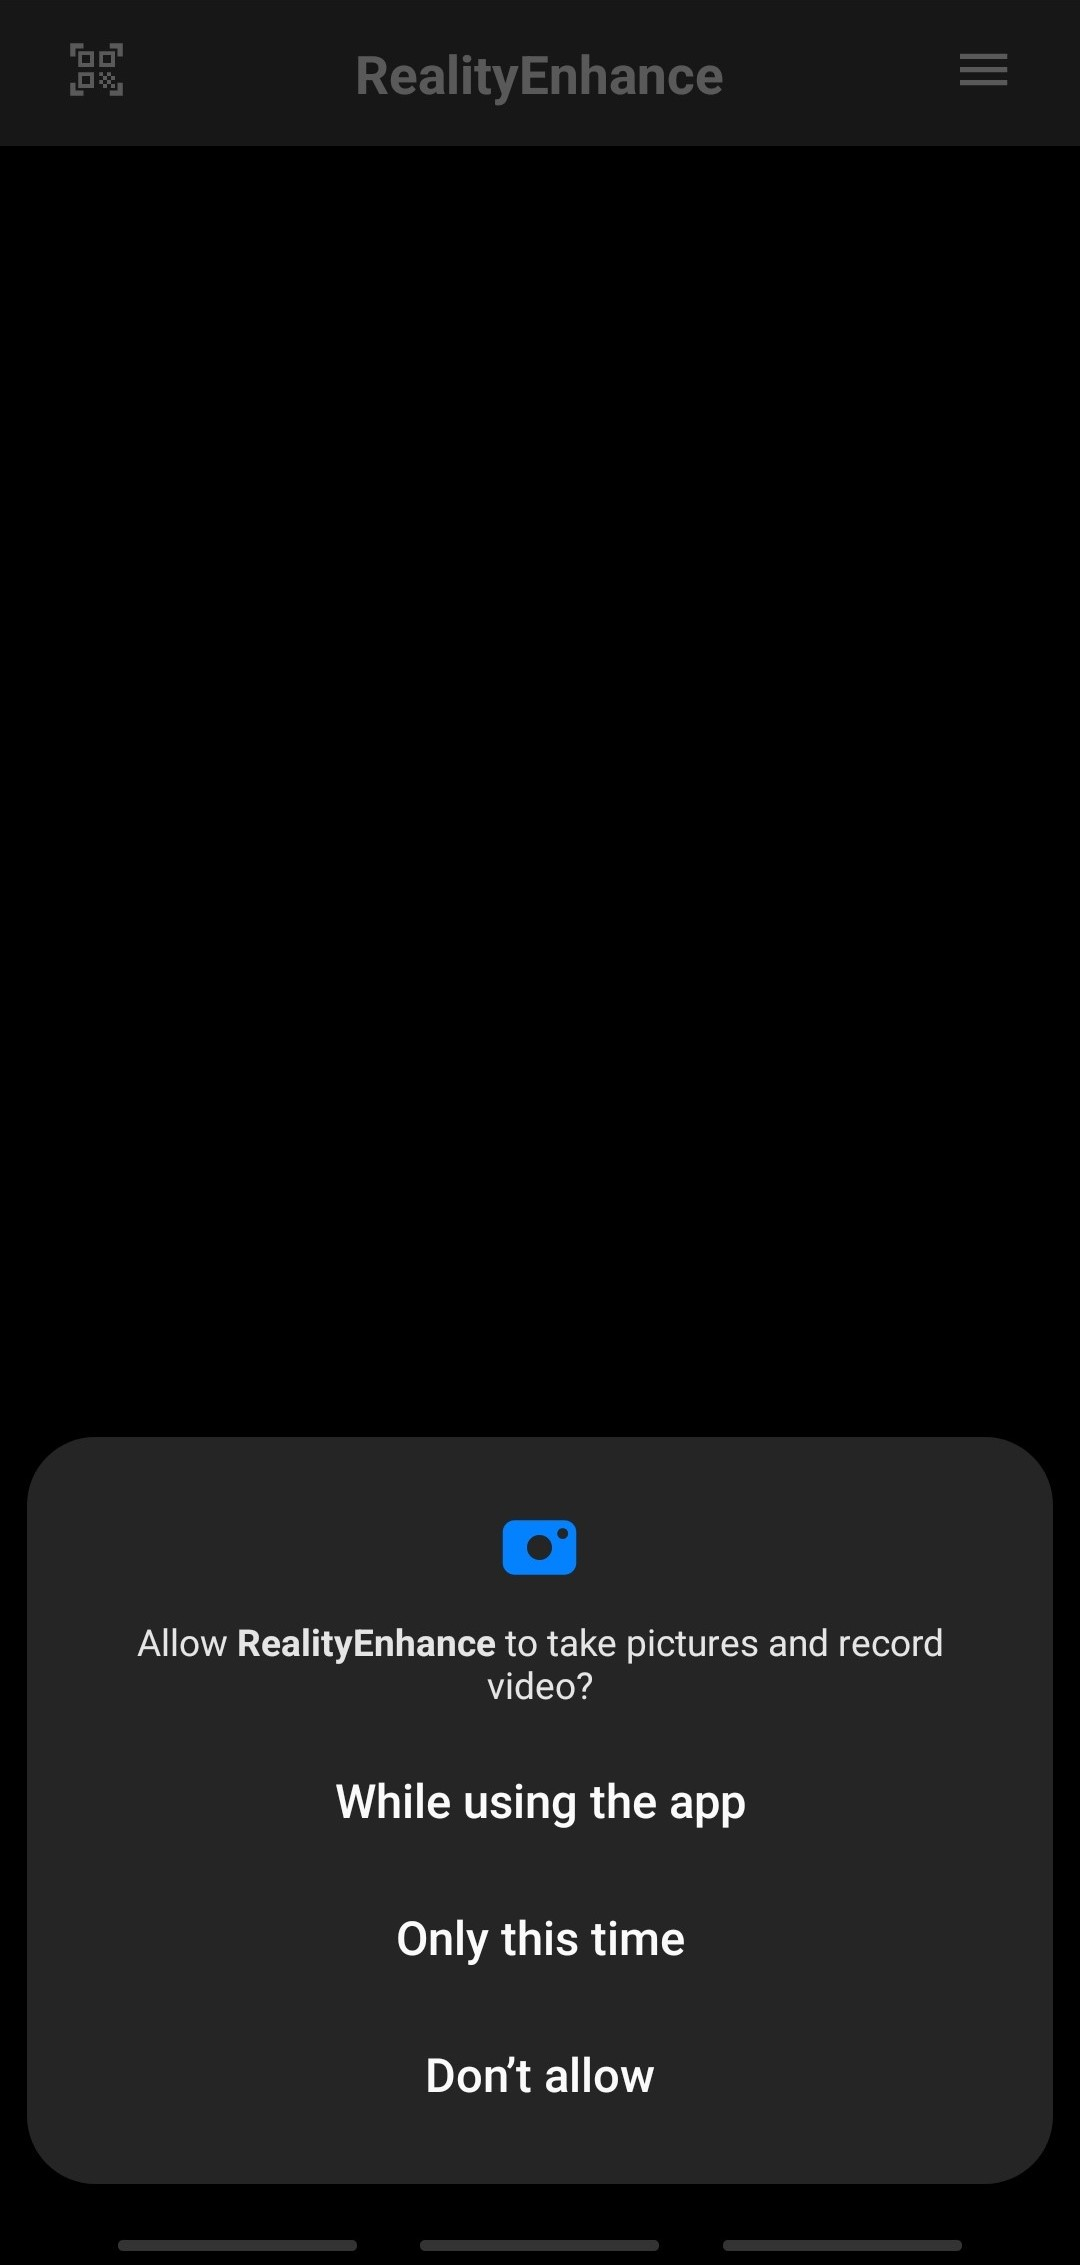
\includegraphics[width=0.4\textwidth]{img/App_screenshots/Ask-for-permission.jpg}}
    \hspace{2cm} % Adjust the horizontal spacing between the images
    \subfigure[Image 2]{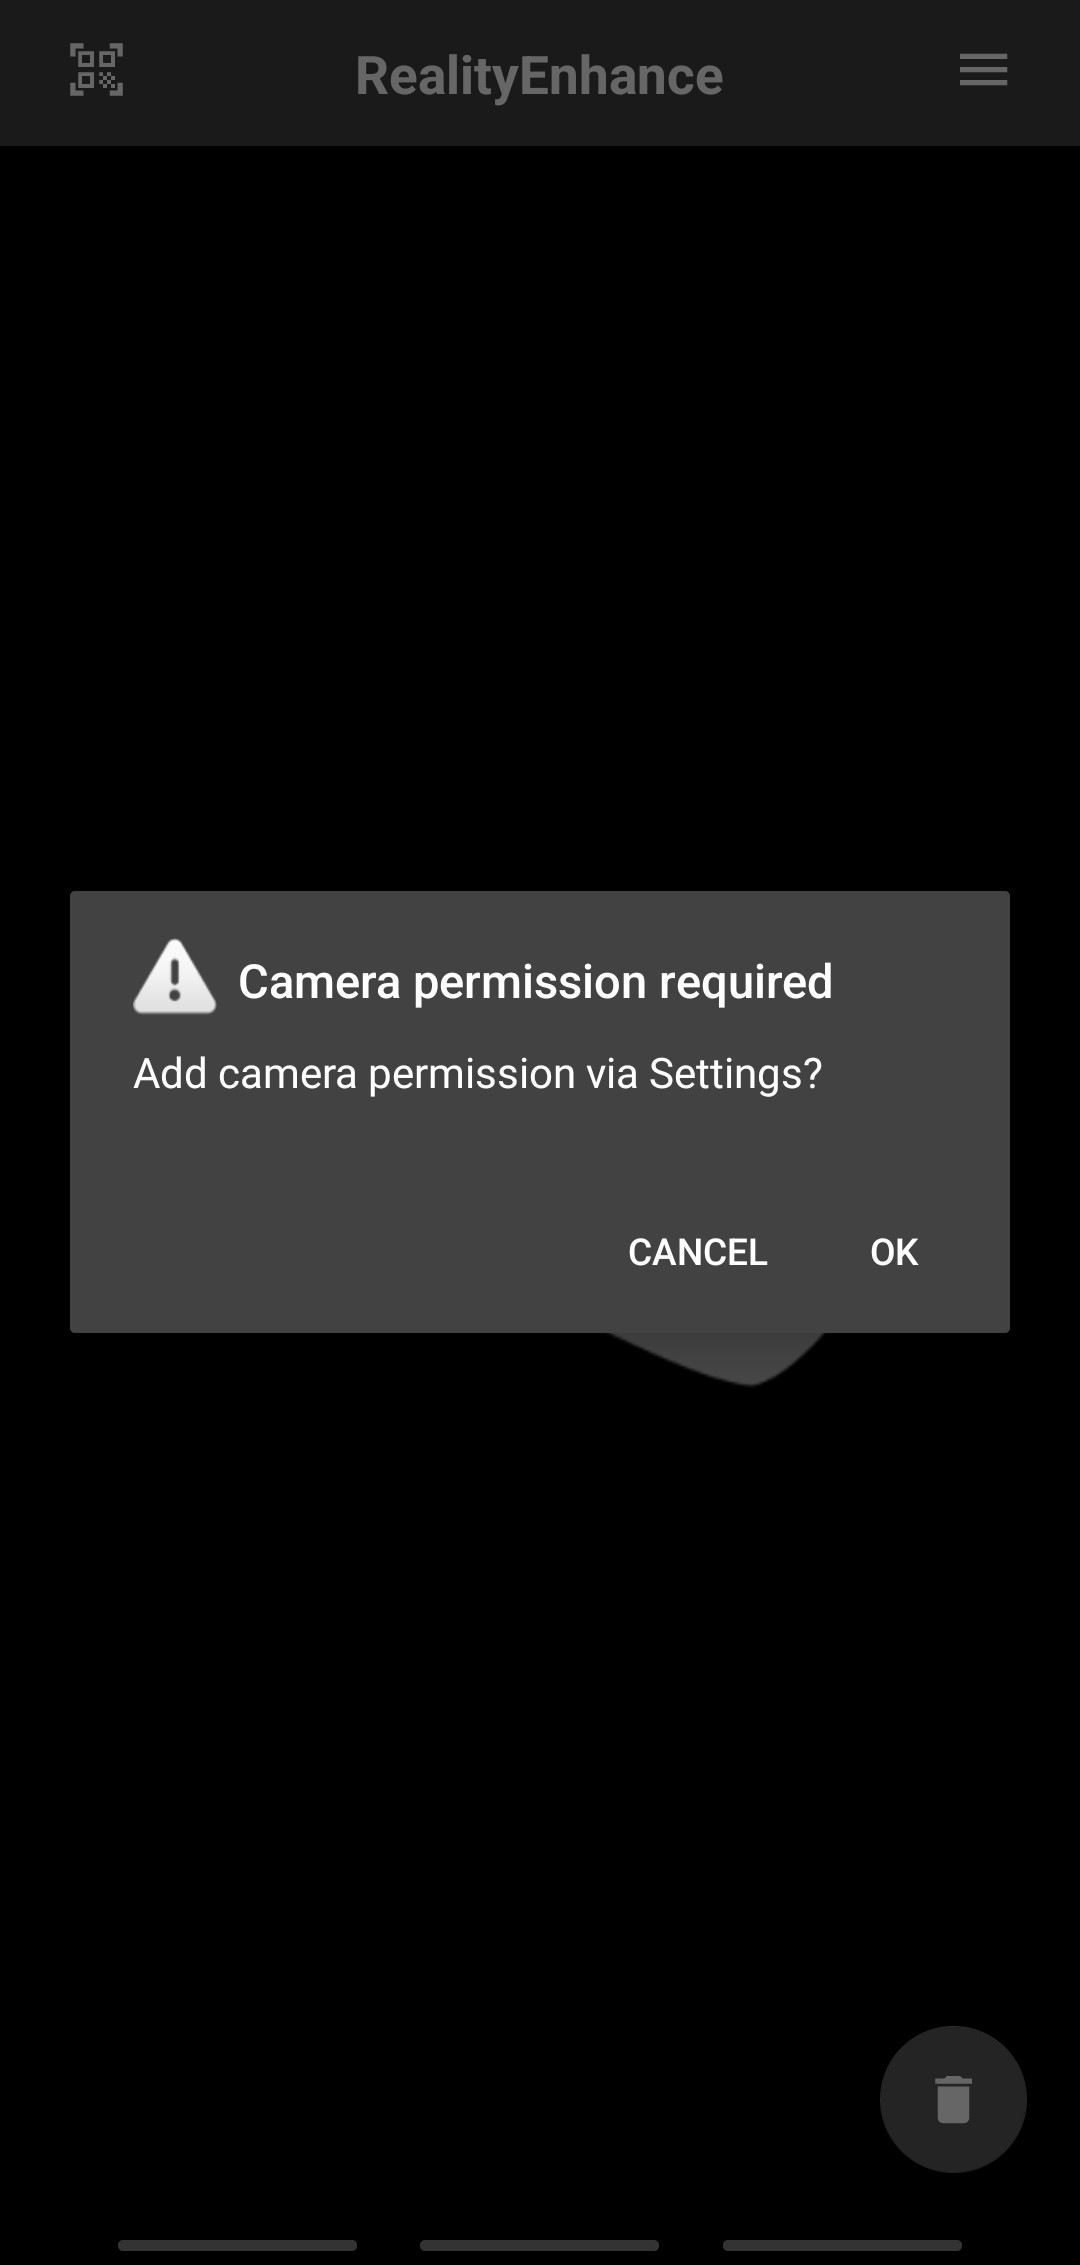
\includegraphics[width=0.4\textwidth]{img/App_screenshots/Camera-permission-required.jpg}}
    \caption{Loading page}
    \label{fig:loading-page}
\end{figure}
\pagebreak


\subsection{Navigation/Tool Bar}
RealityEnhance uses a Navigation/Tool Bar to navigate between the different activities and to access the different features of the app. The application also uses the smartphone's back button (smart gesture from the bottom of the screen or from the sides) to navigate to the previous activity or exit the application. The Navigation/Tool Bar is displayed on the top of the screen. As you can see in Figure \ref{fig:navbar}, the Navigation/Tool Bar has three different modes:

\renewcommand{\labelenumi}{(\alph{enumi})}
\begin{enumerate}
    \item AR Activity  - can access the QR scanner and the Library
    \item QR Activity - can turn on the flashlight and can turn on the auto-focus
    \item Library Activity - can access the QR scanner and the AR Activity
\end{enumerate}

\begin{figure}[ht]
    \begin{center}
        \subfigure[AR Activity]{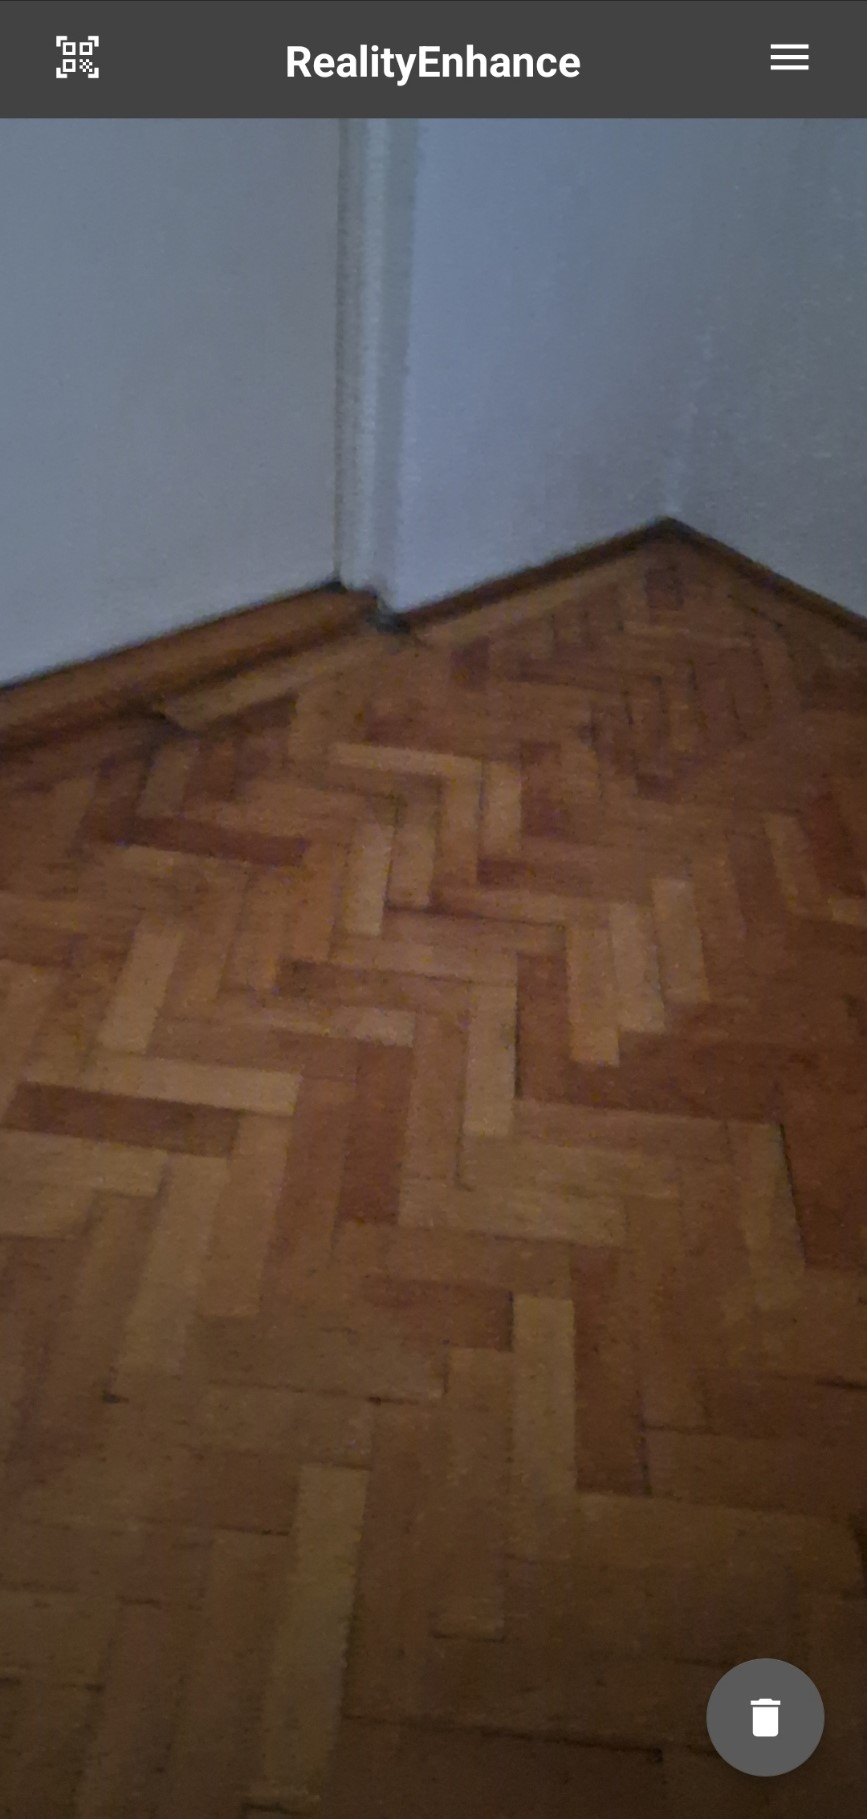
\includegraphics[width=0.3\textwidth]{img/App_screenshots/AR-mode.jpg}}
        \hspace{0.2cm} % Adjust the horizontal spacing between the images
        \subfigure[QR Activity]{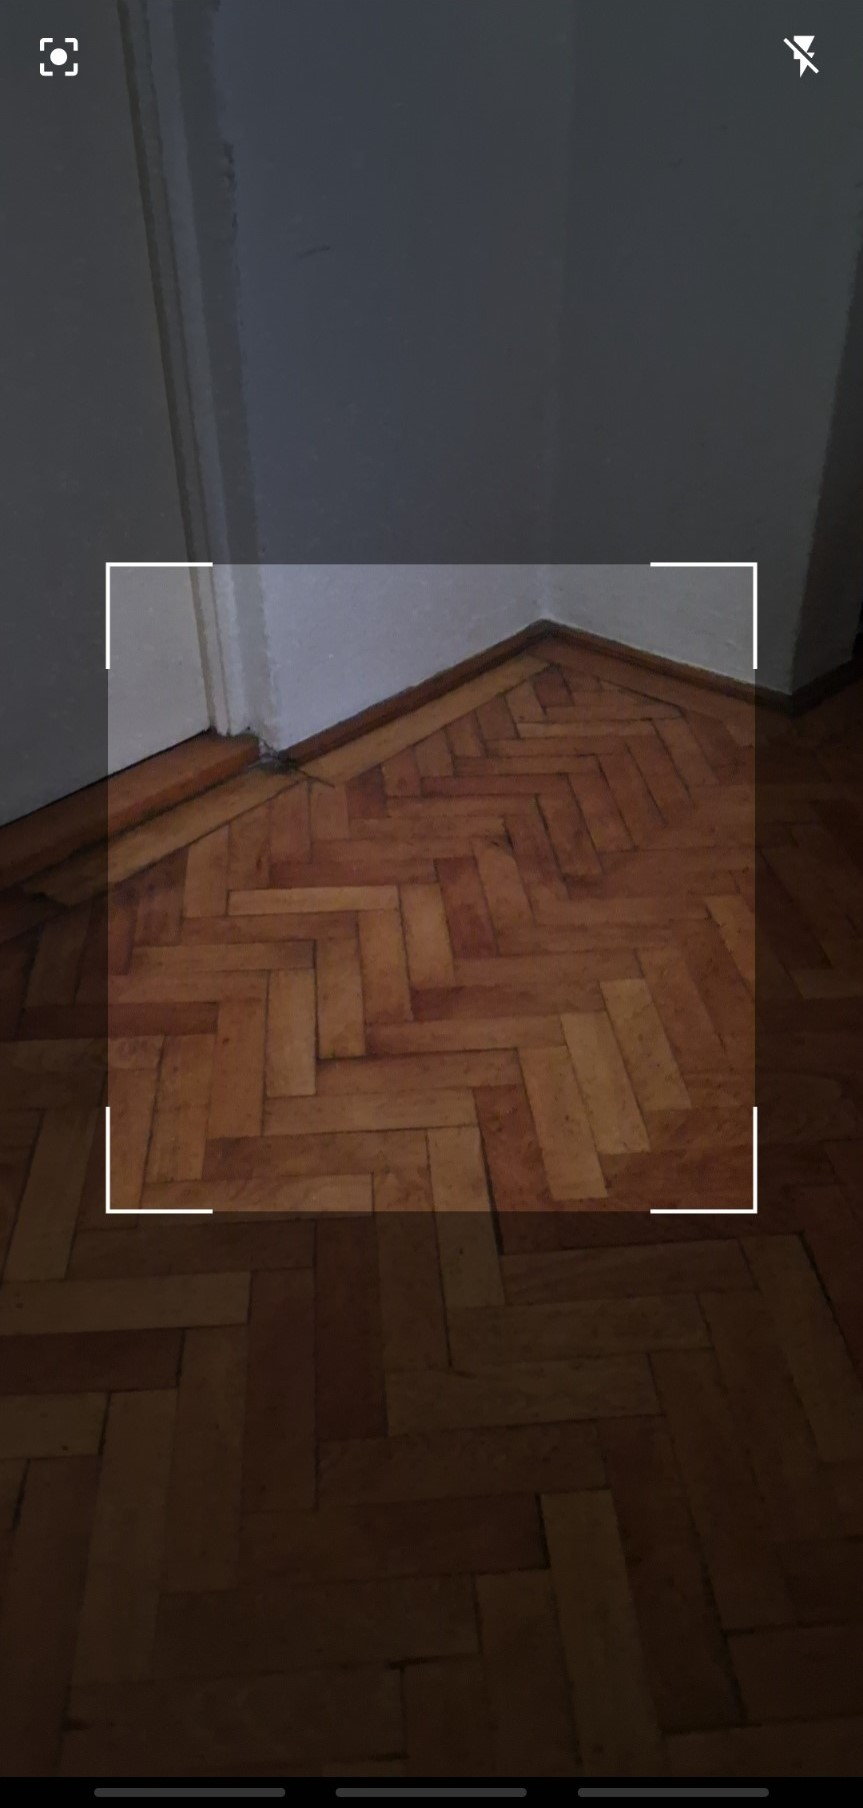
\includegraphics[width=0.3\textwidth]{img/App_screenshots/Scan-QR.jpg}}
        \hspace{0.2cm} % Adjust the horizontal spacing between the images
        \subfigure[Library Activity]{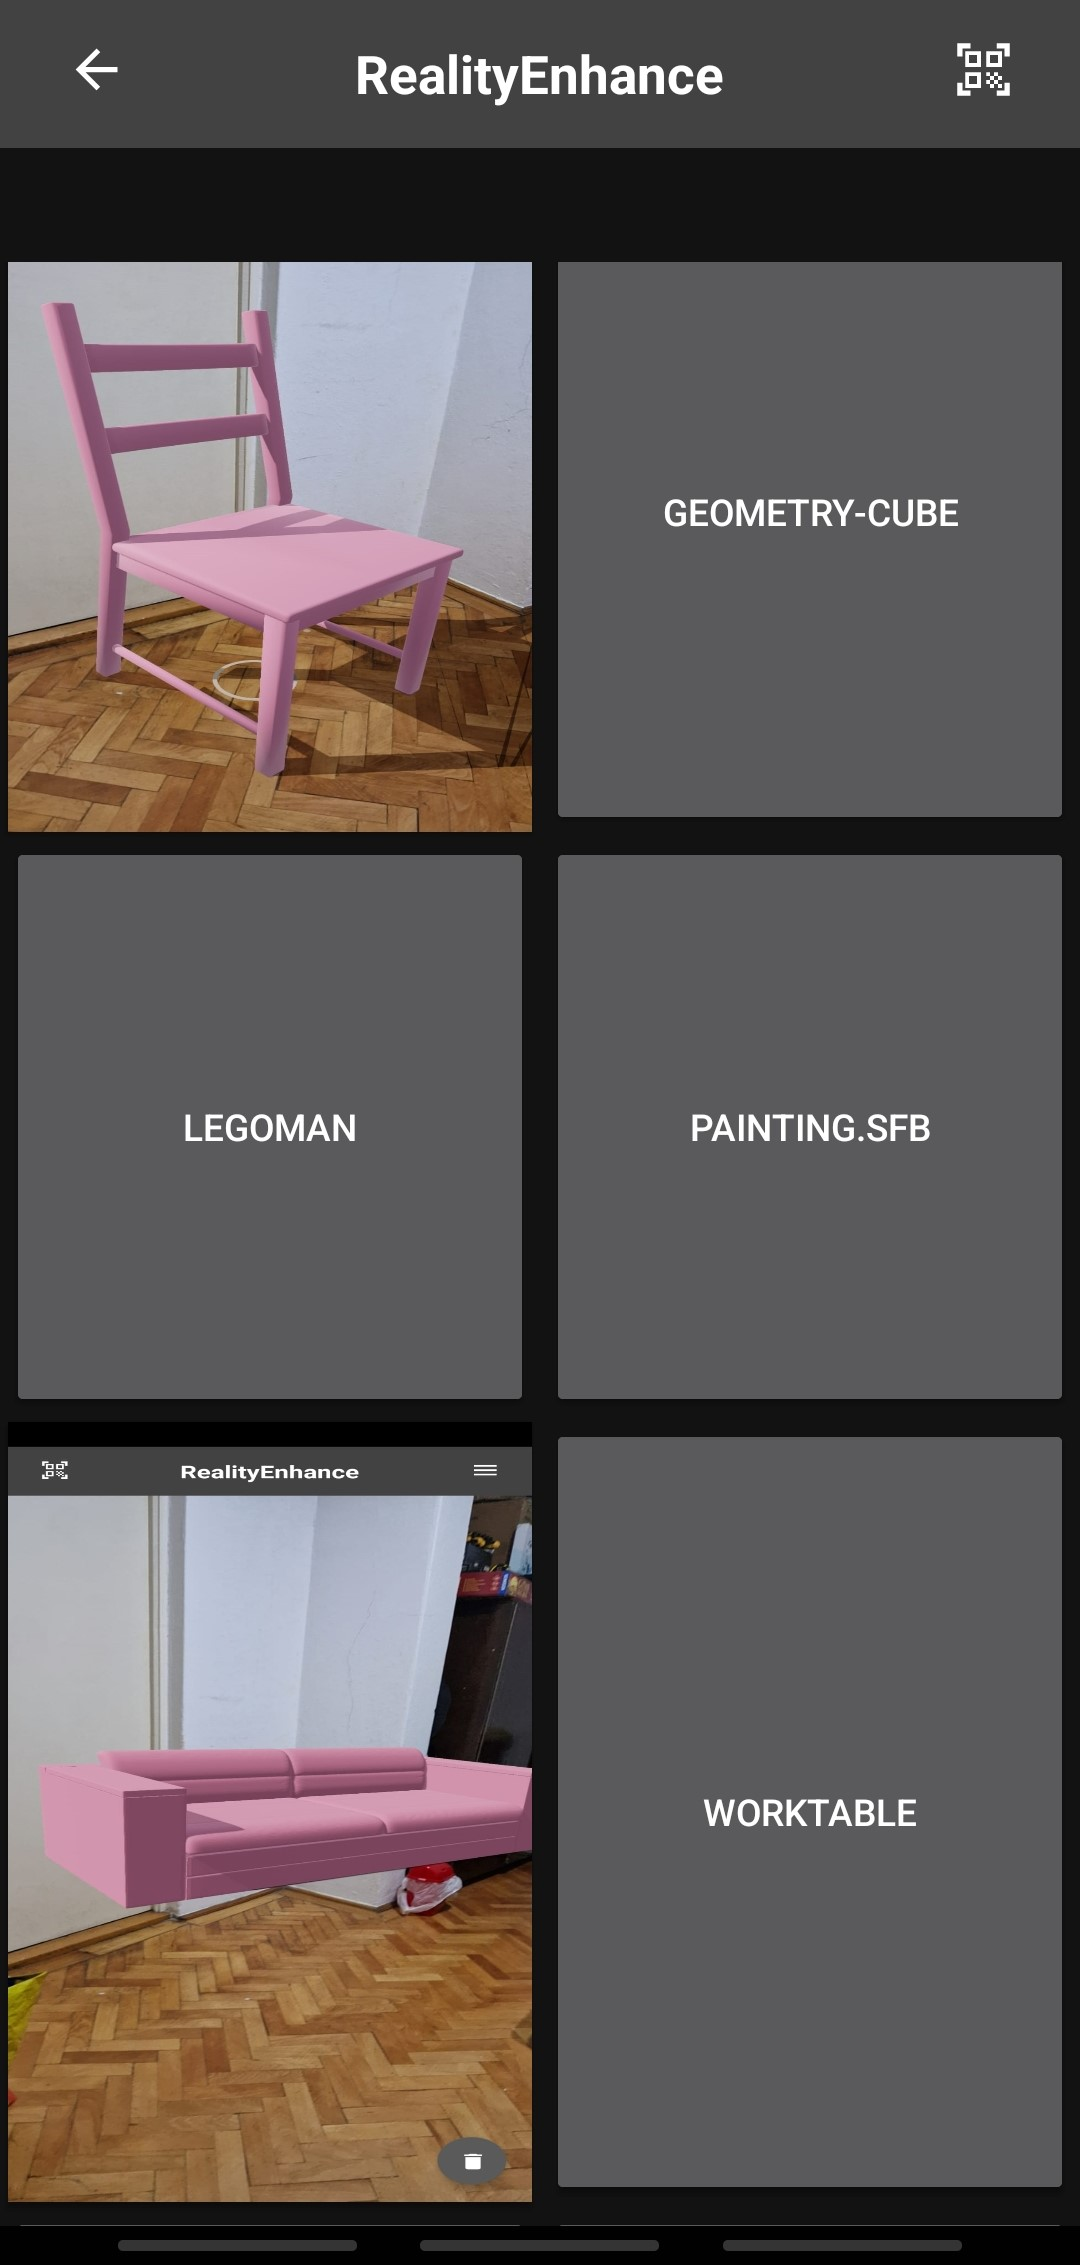
\includegraphics[width=0.3\textwidth]{img/App_screenshots/Library.jpg}}
        \caption{Navigation and toolbar}
        \label{fig:navbar}
    \end{center}
\end{figure}
\pagebreak
\subsection{AR Activity}
The main "page" of the application is the AR activity. This activity is the one that will be displayed when the user launches the application after giving all the permissions. As you can see in Figure \ref{fig:ar-vision} picture \textit{(a)}, an animation of a hand holding a phone will be displayed to indicate the application is scanning the environment and also to indicate to the user how to move the smartphone in order for the surroundings to be scanned.

A scanned surface will be represented by a mesh of dots, as shown in the Figure \ref{fig:ar-vision} picture \textit{(b)}. A surface can be a floor, a table, a wall and many more. The mesh represents the available surfaces the user can place \ac{3D} models.
\begin{figure}[ht]
    \begin{center}
        \subfigure[Scanning animation]{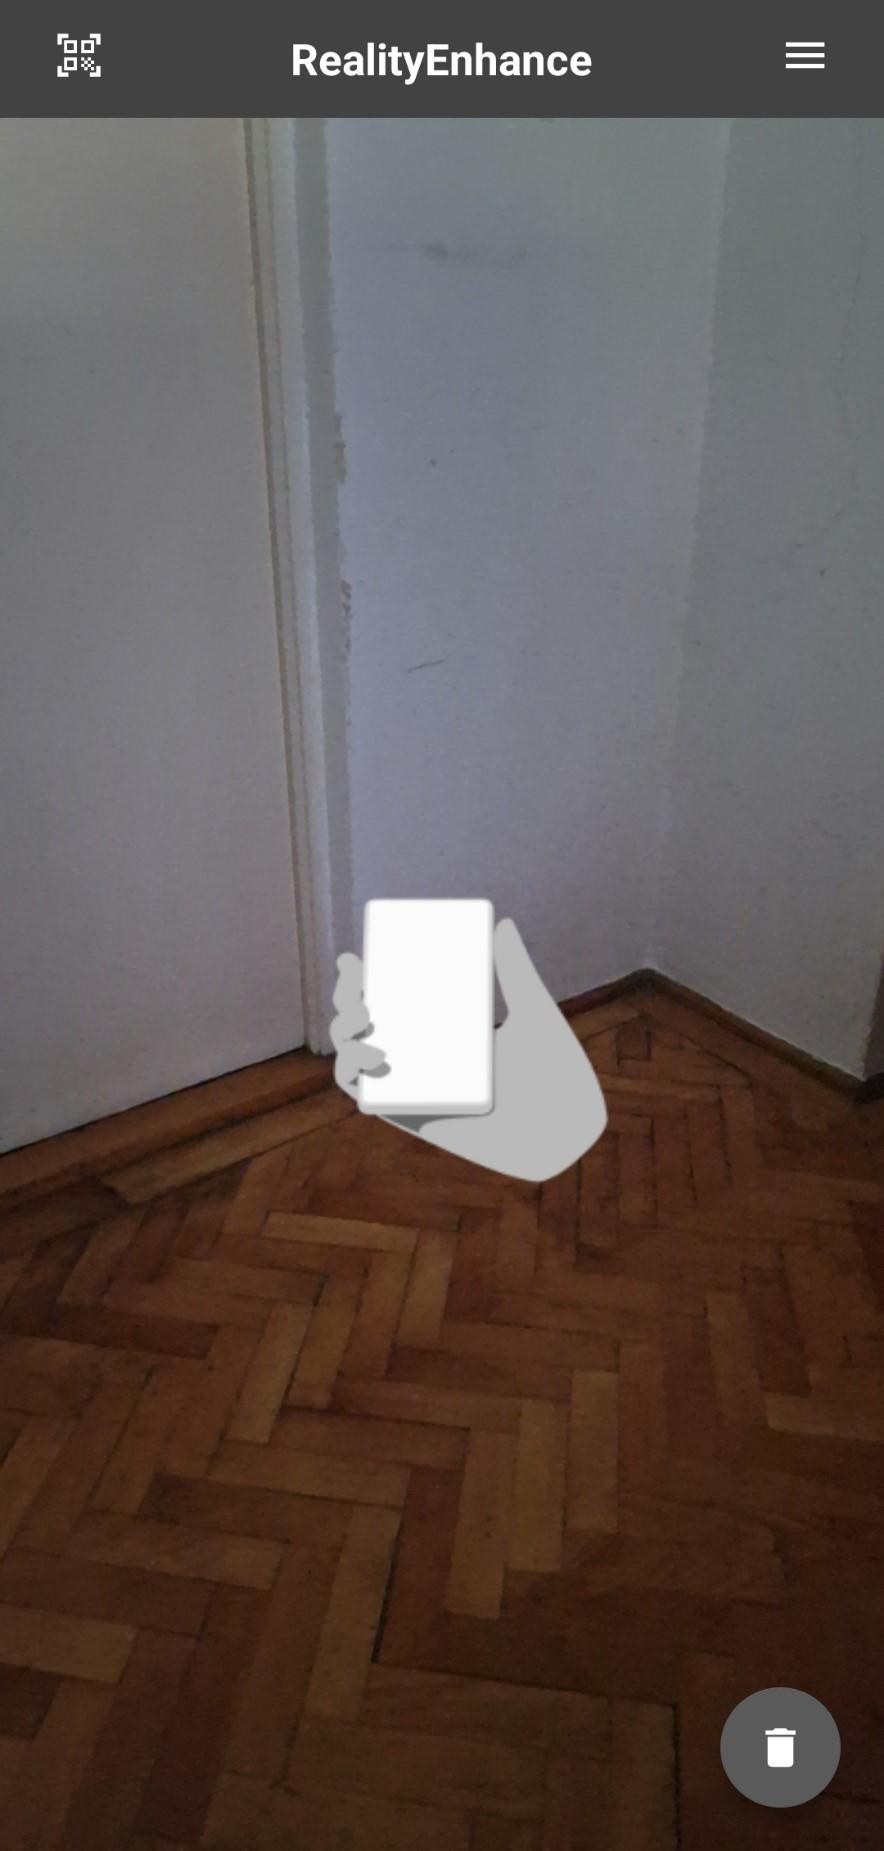
\includegraphics[width=0.4\textwidth]{img/App_screenshots/Scan-enviroment.jpg}}
        \hspace{2cm} % Adjust the horizontal spacing between the images
        \subfigure[Scanned enviroment]{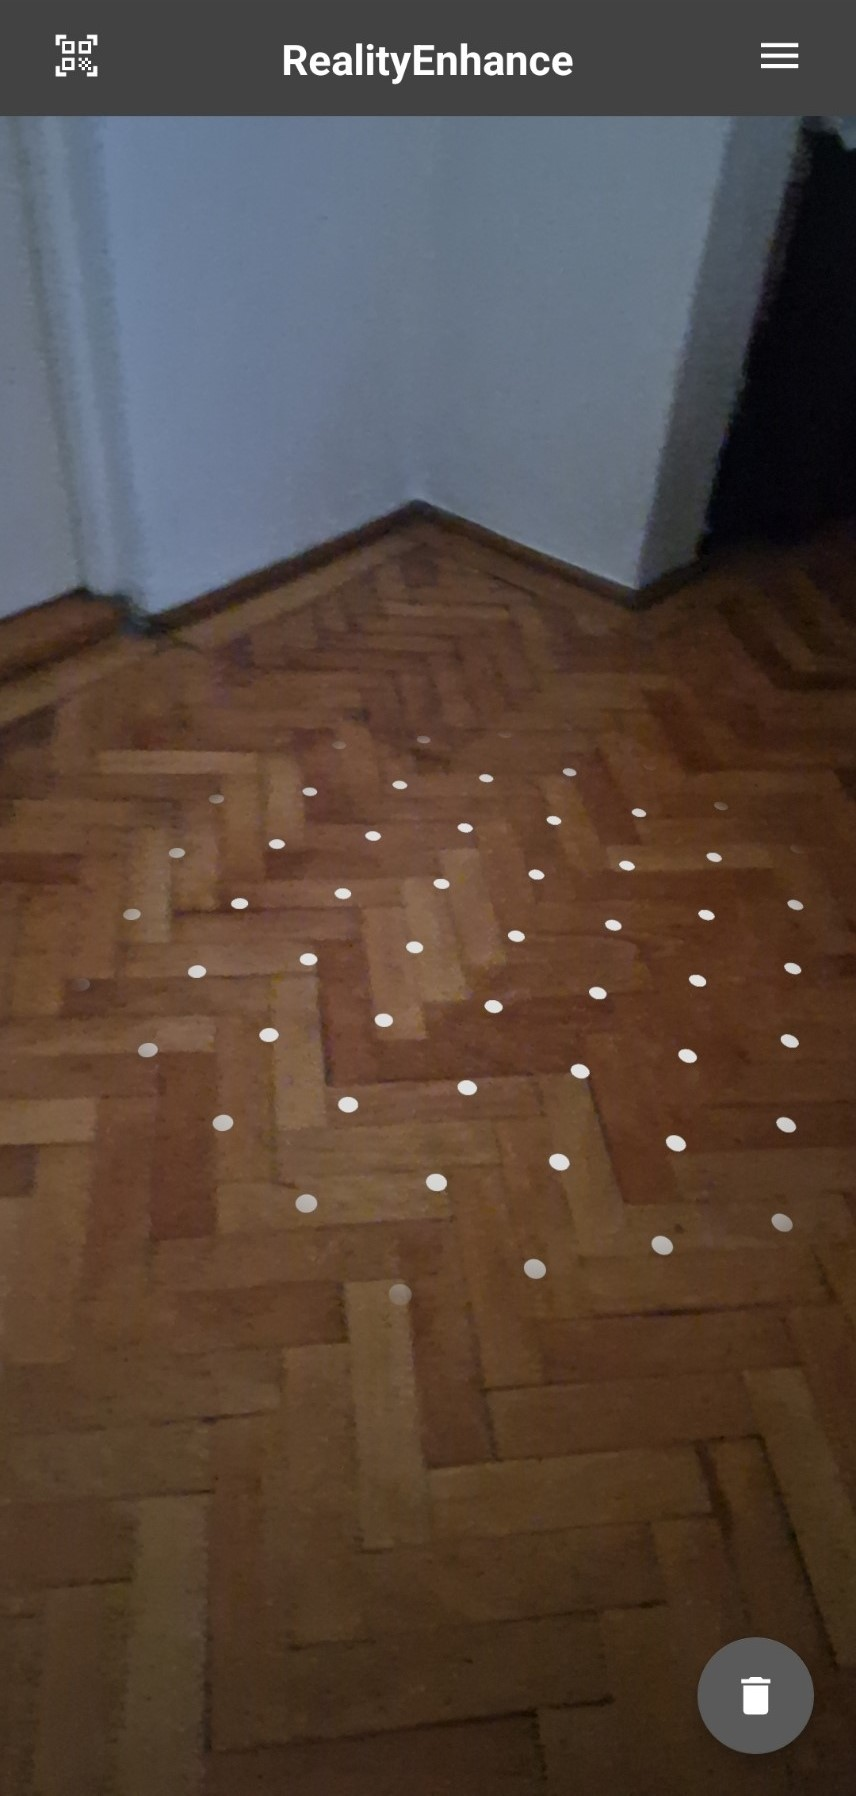
\includegraphics[width=0.4\textwidth]{img/App_screenshots/Scanned-enviromet.jpg}}
        % \hspace{0.2cm} % Adjust the horizontal spacing between the images
        % \subfigure[AR Activity]{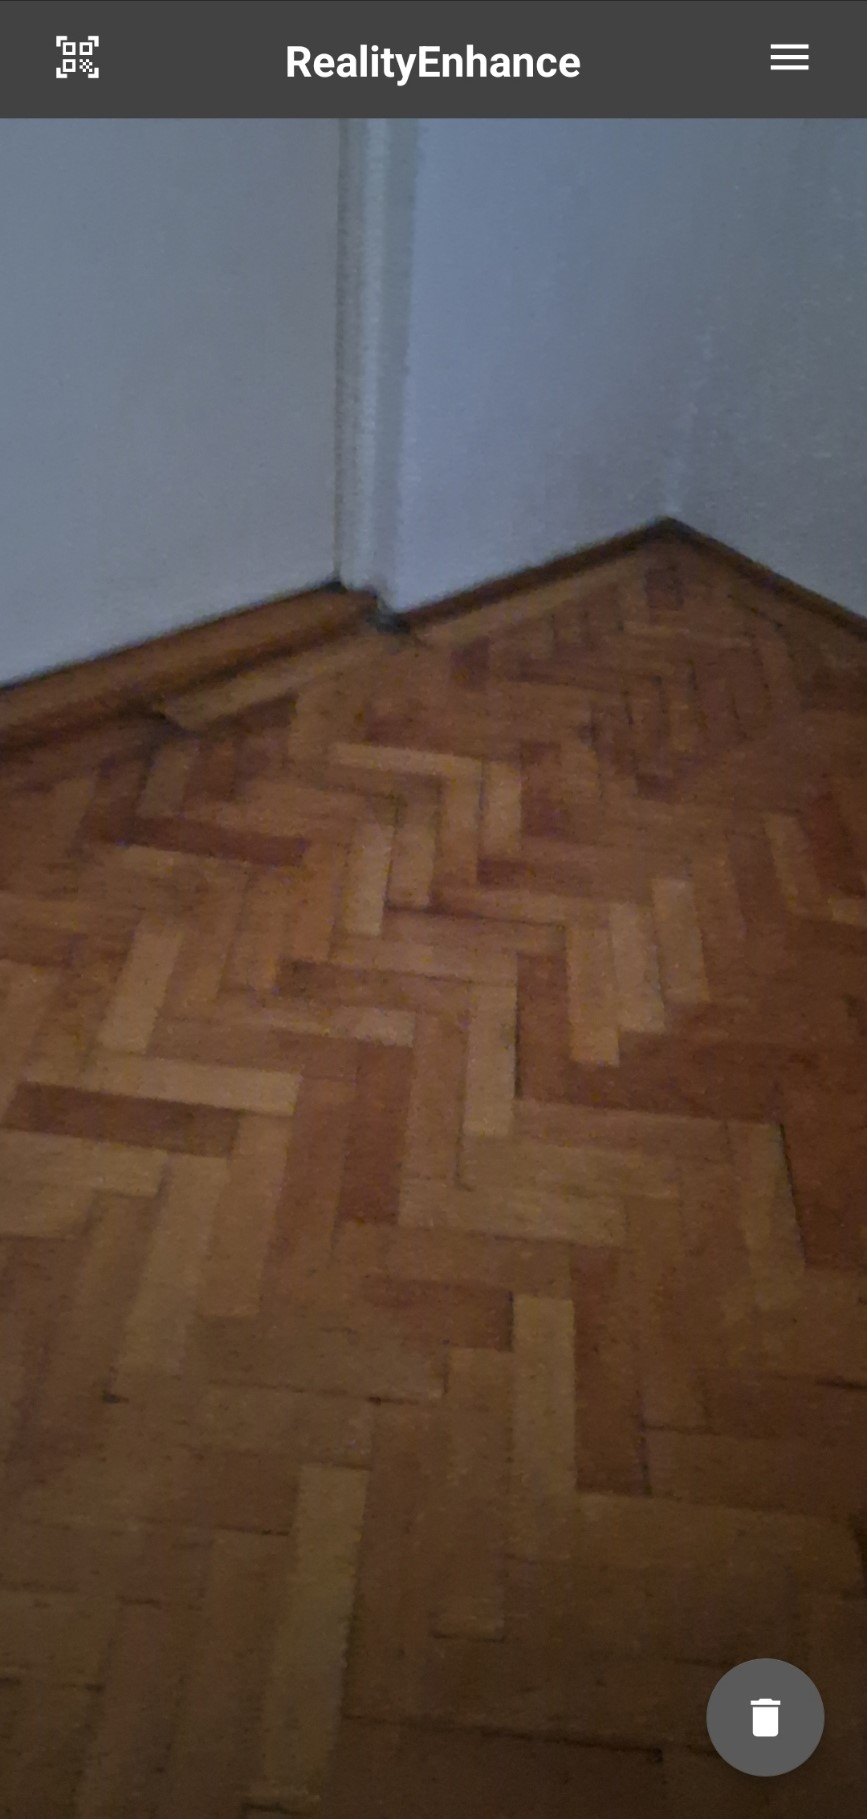
\includegraphics[width=0.3\textwidth]{img/App_screenshots/AR-mode.jpg}}
        \caption{\ac{AR} Activity}
        \label{fig:ar-vision}
    \end{center}
\end{figure}
\pagebreak


\subsection{QR Activity}
The only method to import a new model into the application is by scanning a \ac{QR} code. In  Figure \ref{fig:qr-scanner}, we can see the interface of the scanner. To scan a \ac{QR} code, the user needs to point the camera to the \ac{QR} code and fit the code in the square. The scanner will automatically scan the code and will load the model in the application. The user will then be redirected to the AR Activity.

The user can also turn on the flashlight and the auto-focus by clicking on the buttons on the top of the screen. If the QR code is invalid, the user will be notified by a pop-up message, and the scanner will be restarted.

\begin{figure}[ht]
    \begin{center}
        \subfigure[QR Activity]{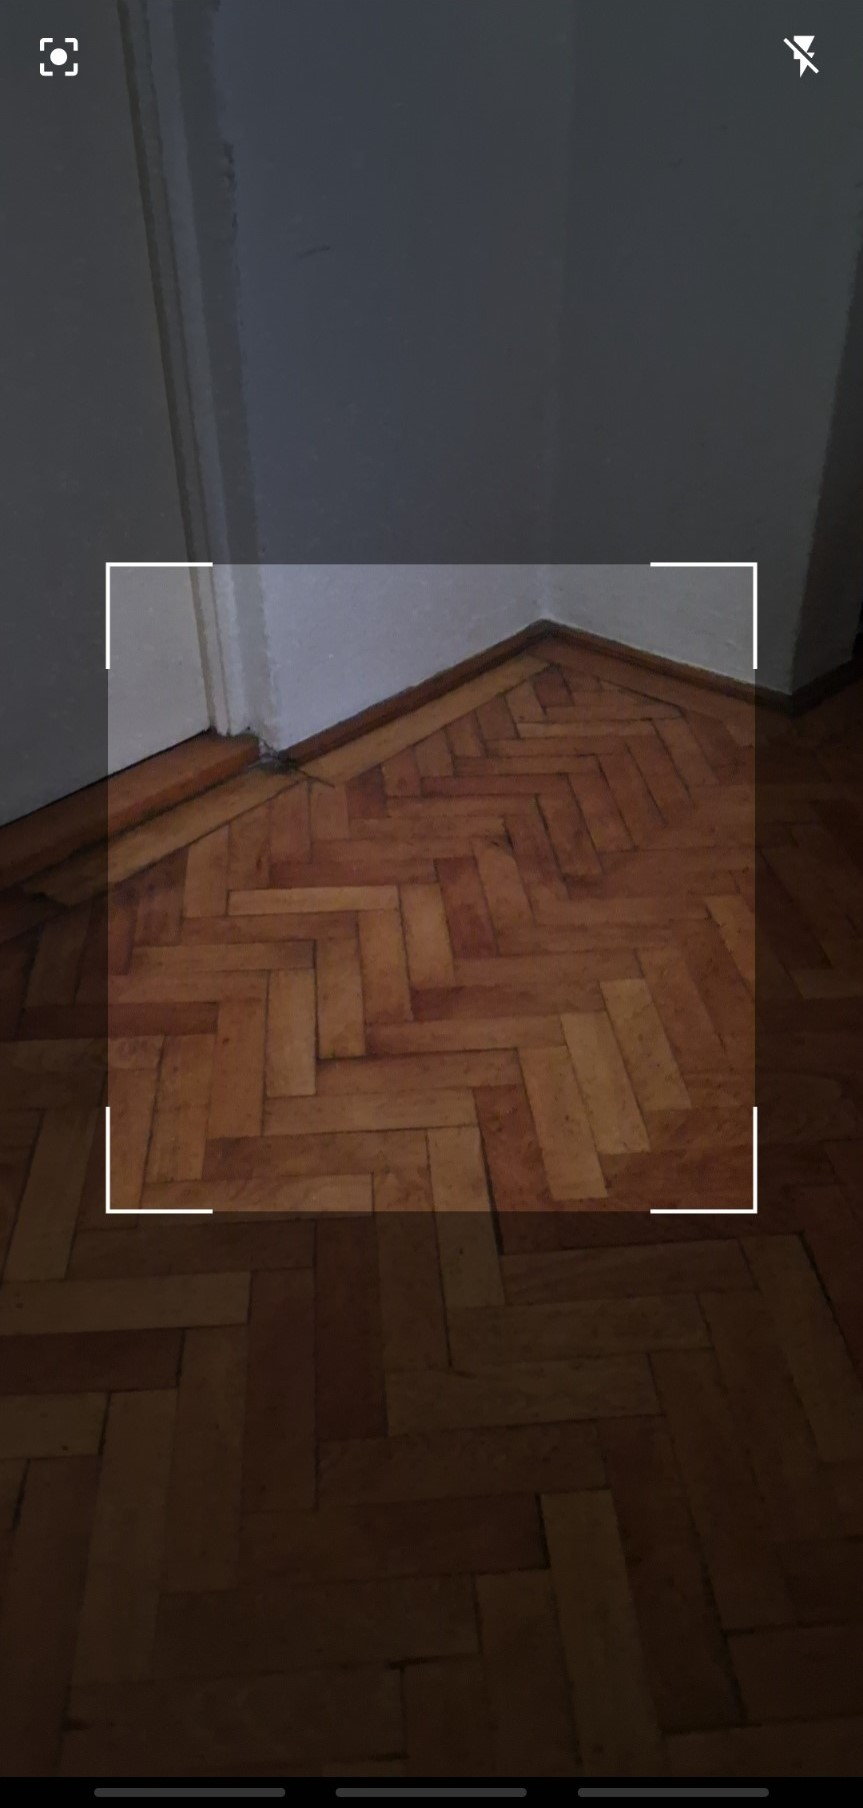
\includegraphics[width=0.4\textwidth]{img/App_screenshots/Scan-QR.jpg}}
        \hspace{2cm} % Adjust the horizontal spacing between the images
        \subfigure[Scanning QR code]{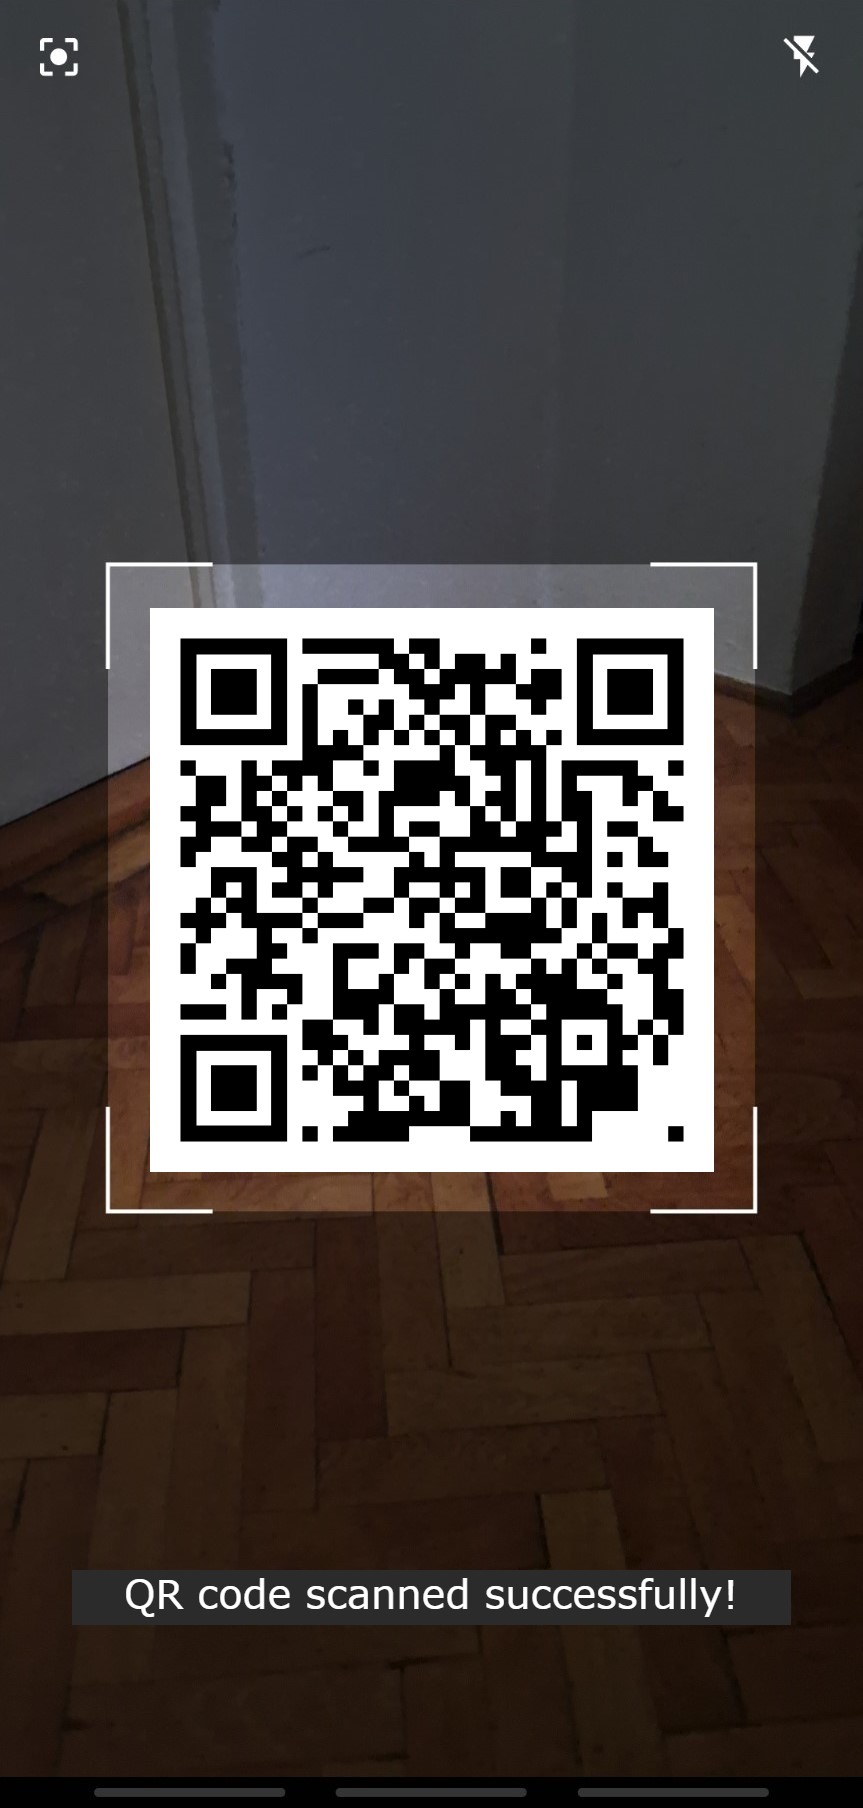
\includegraphics[width=0.4\textwidth]{img/App_screenshots/Scanning-QR.png}}
        \caption{\ac{QR} Activity}
        \label{fig:qr-scanner}
    \end{center}
\end{figure}
\pagebreak

\subsection{Library Activity}
RealityEnhance has, from the start, a couple of \ac{3D} models preloaded in the library. The user can access the library by clicking on the library button (the button is represented by three  lines) in the Navigation/Tool Bar. As you can observe in Figure \ref{fig:library}, the library has a grid listing of models that the user can choose from.

The user can click on a model to load it into the application. The user will then need to go back to the AR Activity to use the model. From the library, the user can also access the QR scanner by clicking on the QR button (the button is represented by a QR code). The list of models is scrollable, and the user can scroll through the list by swiping up or down on the screen.

\begin{figure}[ht]
    \begin{center}
        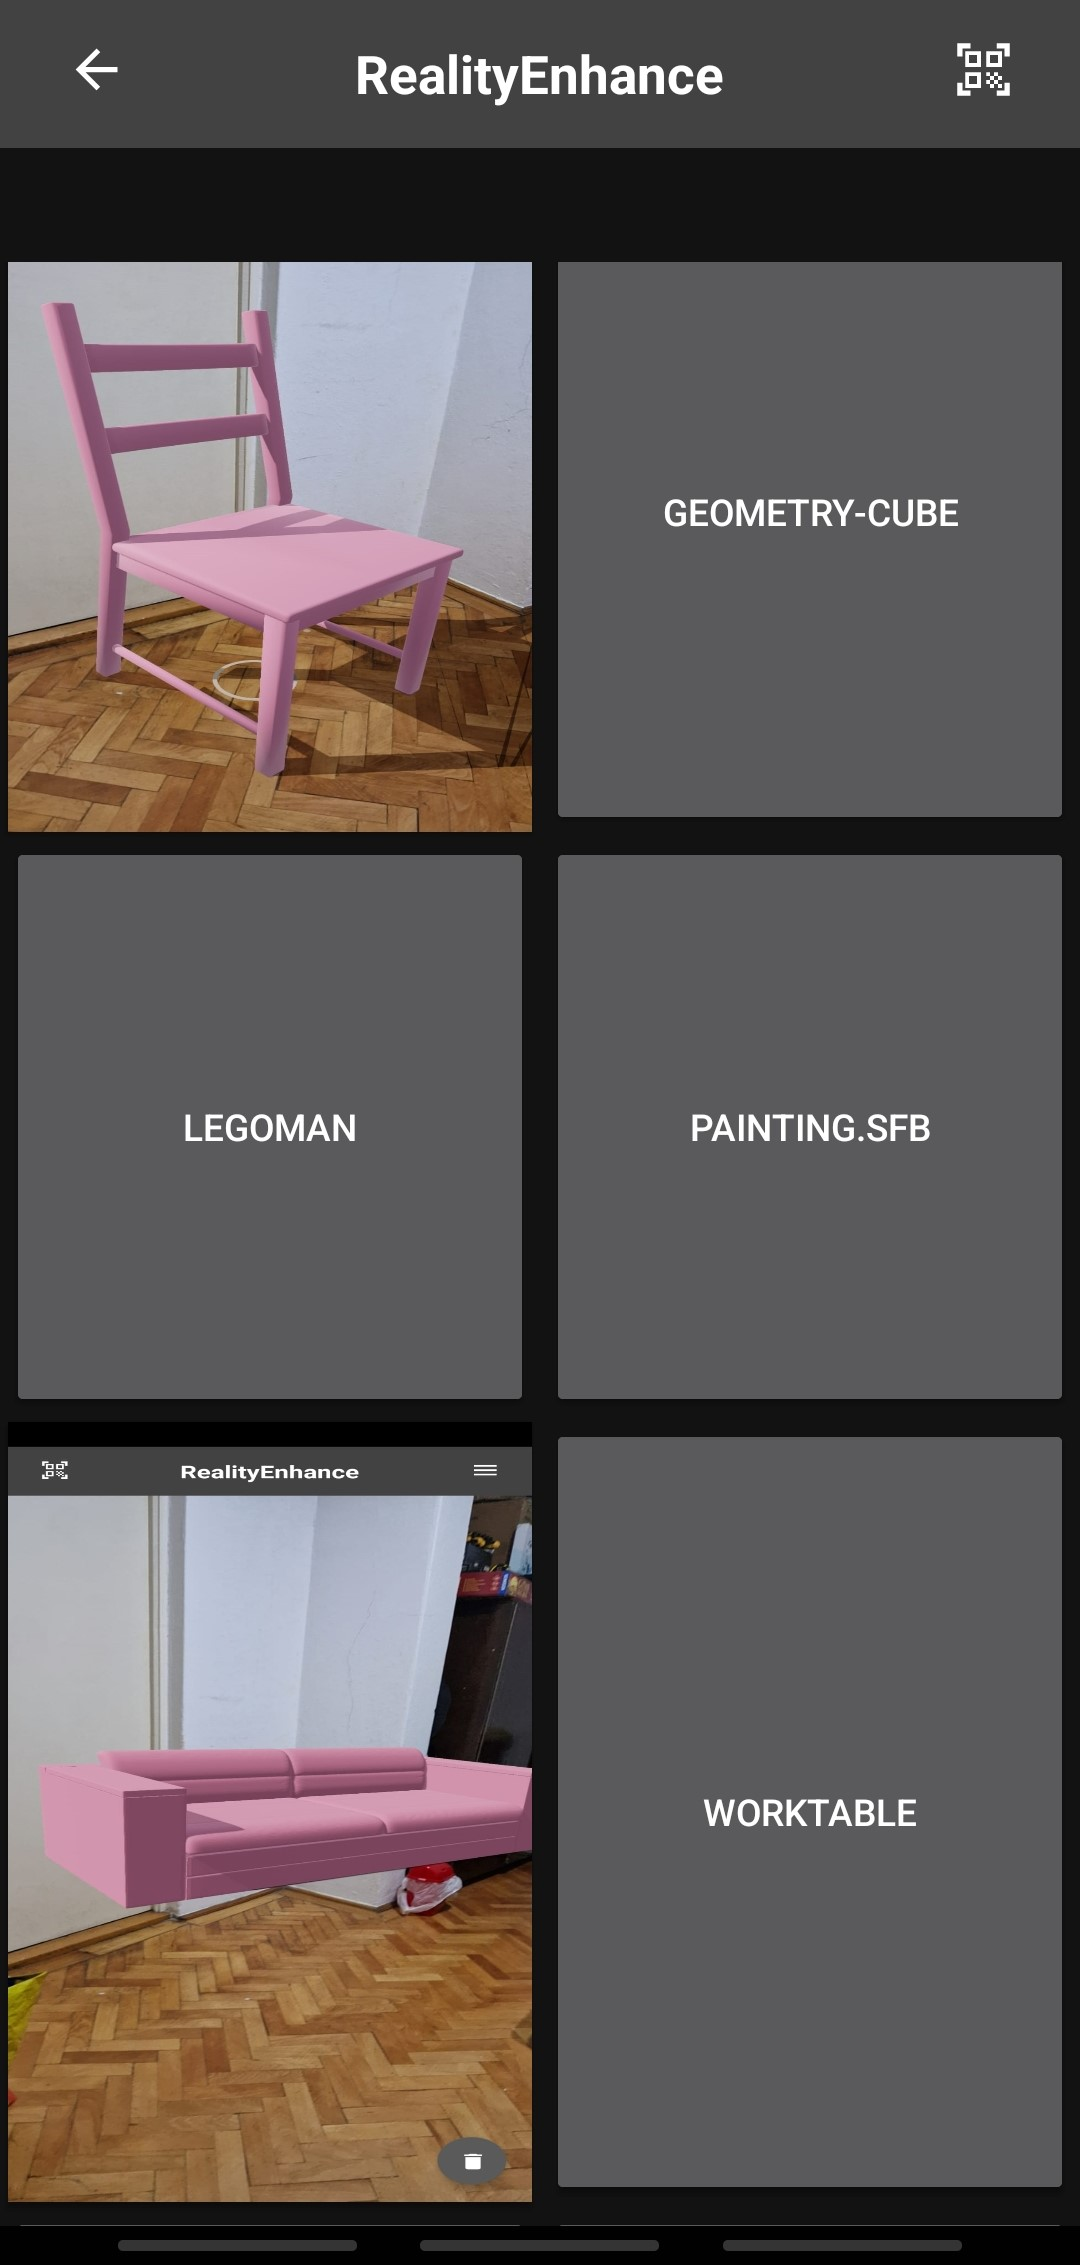
\includegraphics[width=0.4\textwidth]{img/App_screenshots/Library.jpg}
        \caption{Library Activity}
        \label{fig:library}
    \end{center}
\end{figure}
\pagebreak

\subsection{Placing a model}

After the user has either scanned a model or selected one from the library, the user can place the model in the environment (on the scanned surface), as shown in Figure \ref{fig:placed-model}. The model's placement is done by simply touching the screen at the desired location.

Users are not limited to a single model. They can add multiple models to the scene, the same model or different models. The position of the already placed model will be maintained even if the user changes the activity or change the application they are using. In order to know which model is selected, the user can see a white circle under the model.
\begin{figure}[ht]
    \begin{center}
        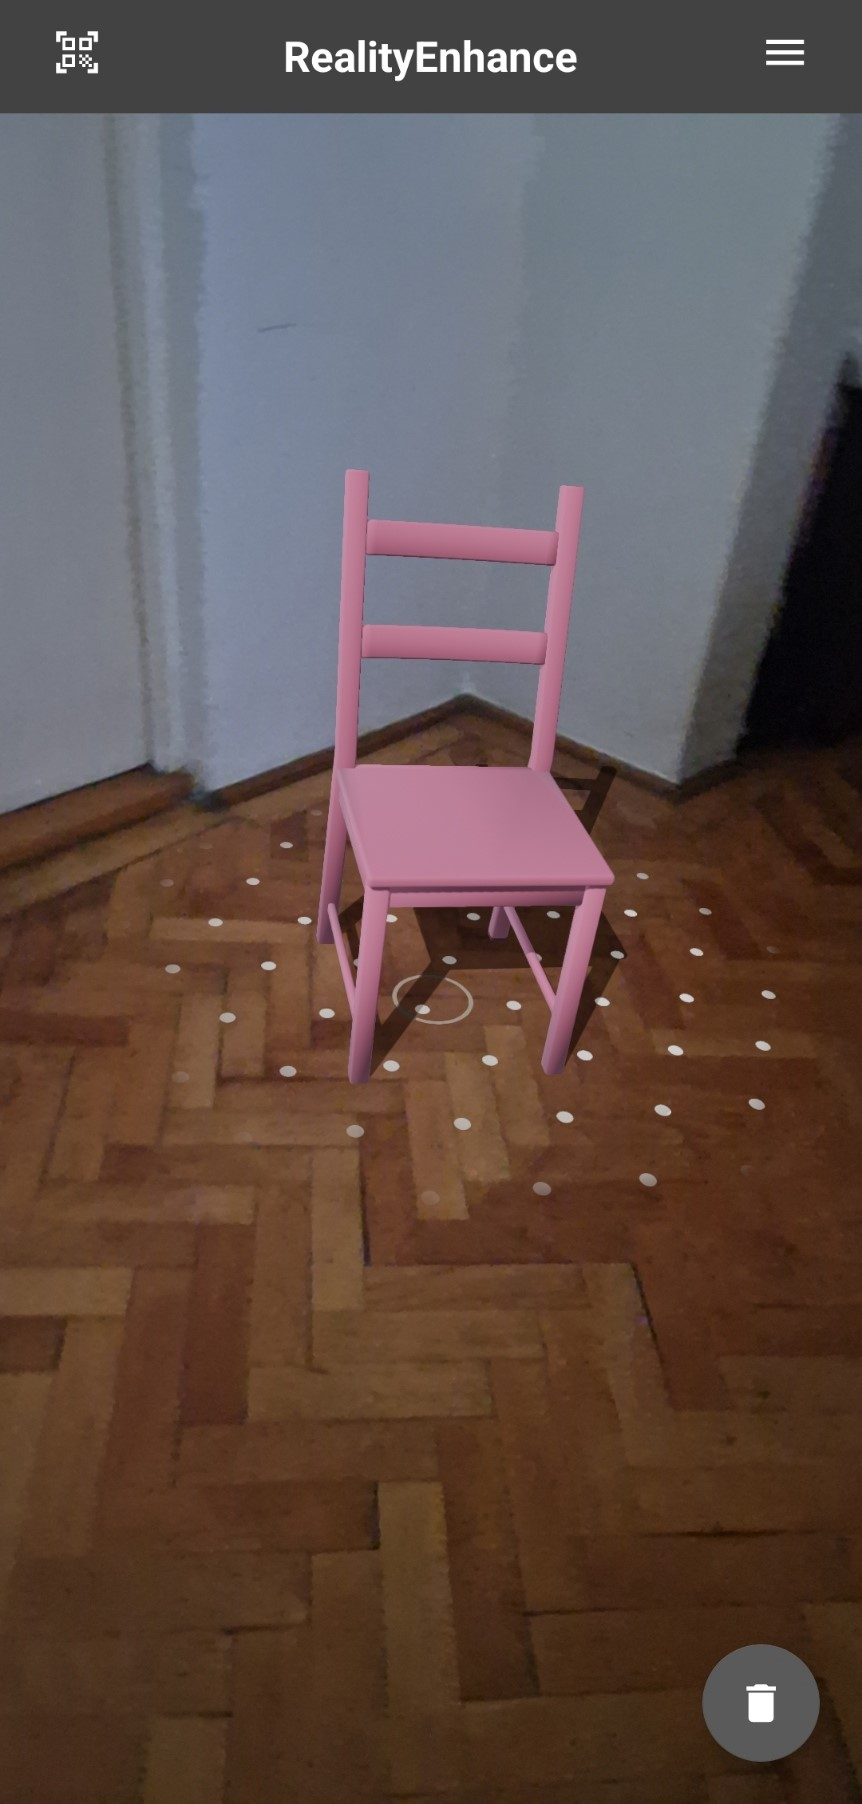
\includegraphics[width=0.4\textwidth]{img/App_screenshots/Model-placed.jpg}
        \caption{Placing a model}
        \label{fig:placed-model}
    \end{center}
\end{figure}
\pagebreak

\subsection{Using multiple models at the same time}
The user will be able to use multiple models at the same time in the same scene. The model's hitboxes will be separated, and the user will be able to select a model by clicking on it, but the models will not interact with each other.

The only interaction between models is that they can cast shadows on one another. The user can see in Figure \ref{fig:multiple-models} an example of multiple models placed in the same scene and that the worktable is casting a shadow on the chair.

\begin{figure}[ht]
    \begin{center}
        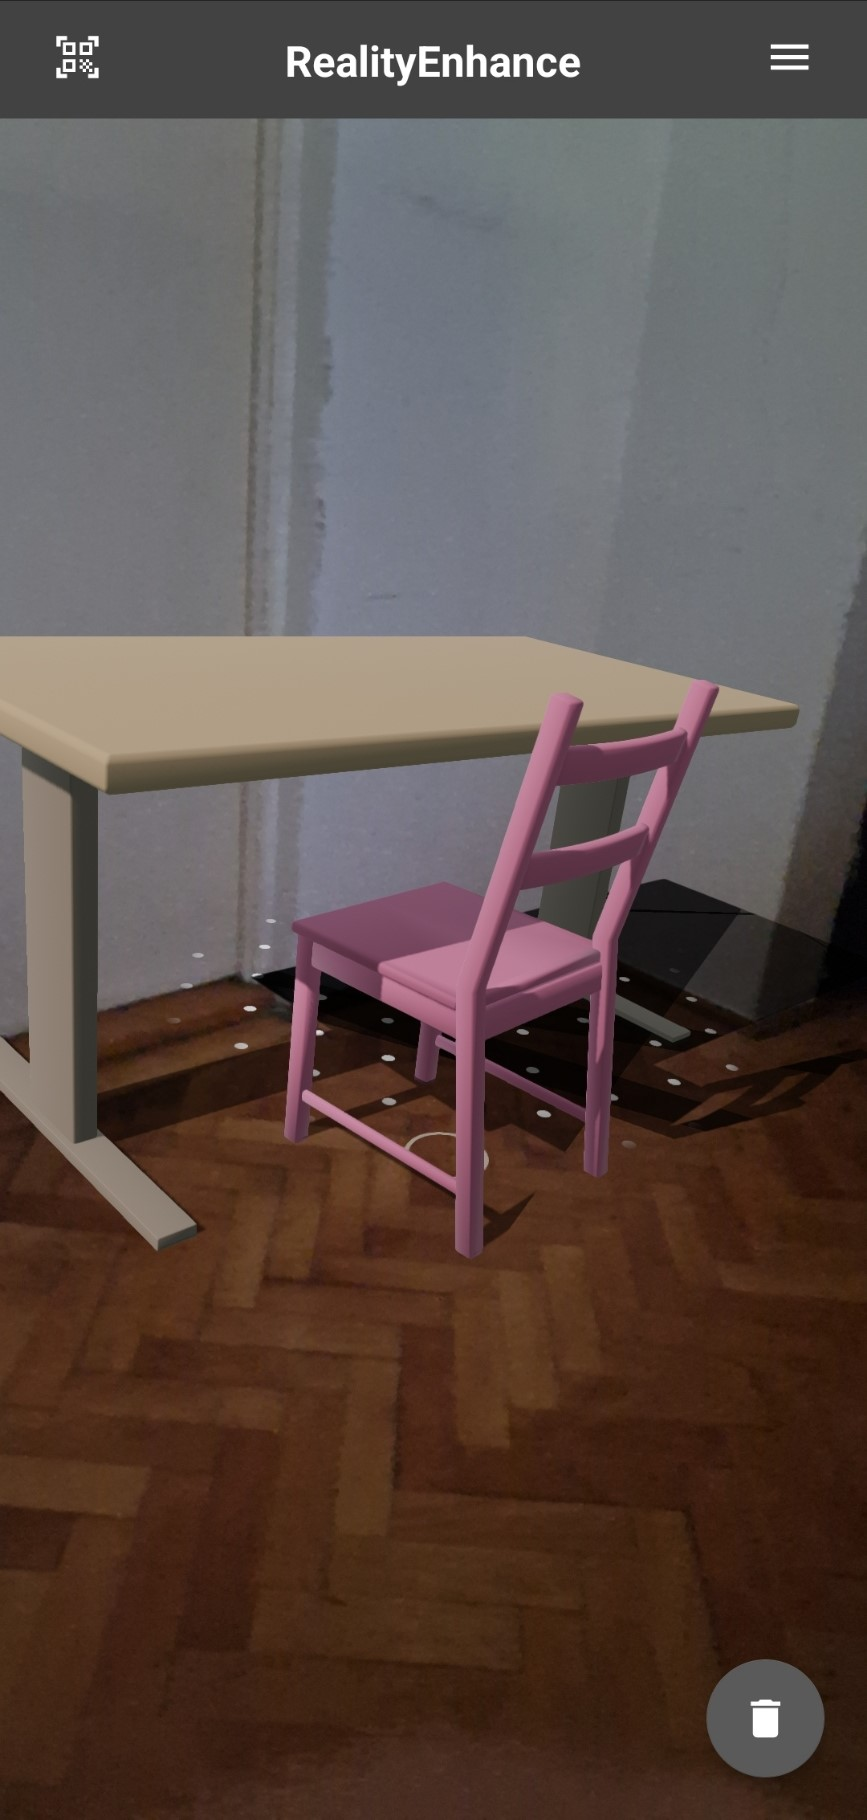
\includegraphics[width=0.5\textwidth]{img/App_screenshots/Multiple-models.jpg}
        \caption{Removing a model}
        \label{fig:multiple-models}
    \end{center}
\end{figure}
\pagebreak

\subsection{Removing a model}
The user can remove the model by selecting it by clicking and then pressing the delete button. The delete button is represented by a trash can icon in the bottom right of the screen. The user can also remove a model by clicking and dragging the model on top of the delete button. The user can also remove all the models placed by holding the delete button for 5 seconds.\ref{fig:remove-a-model}.

\begin{figure}[ht]
    \begin{center}
        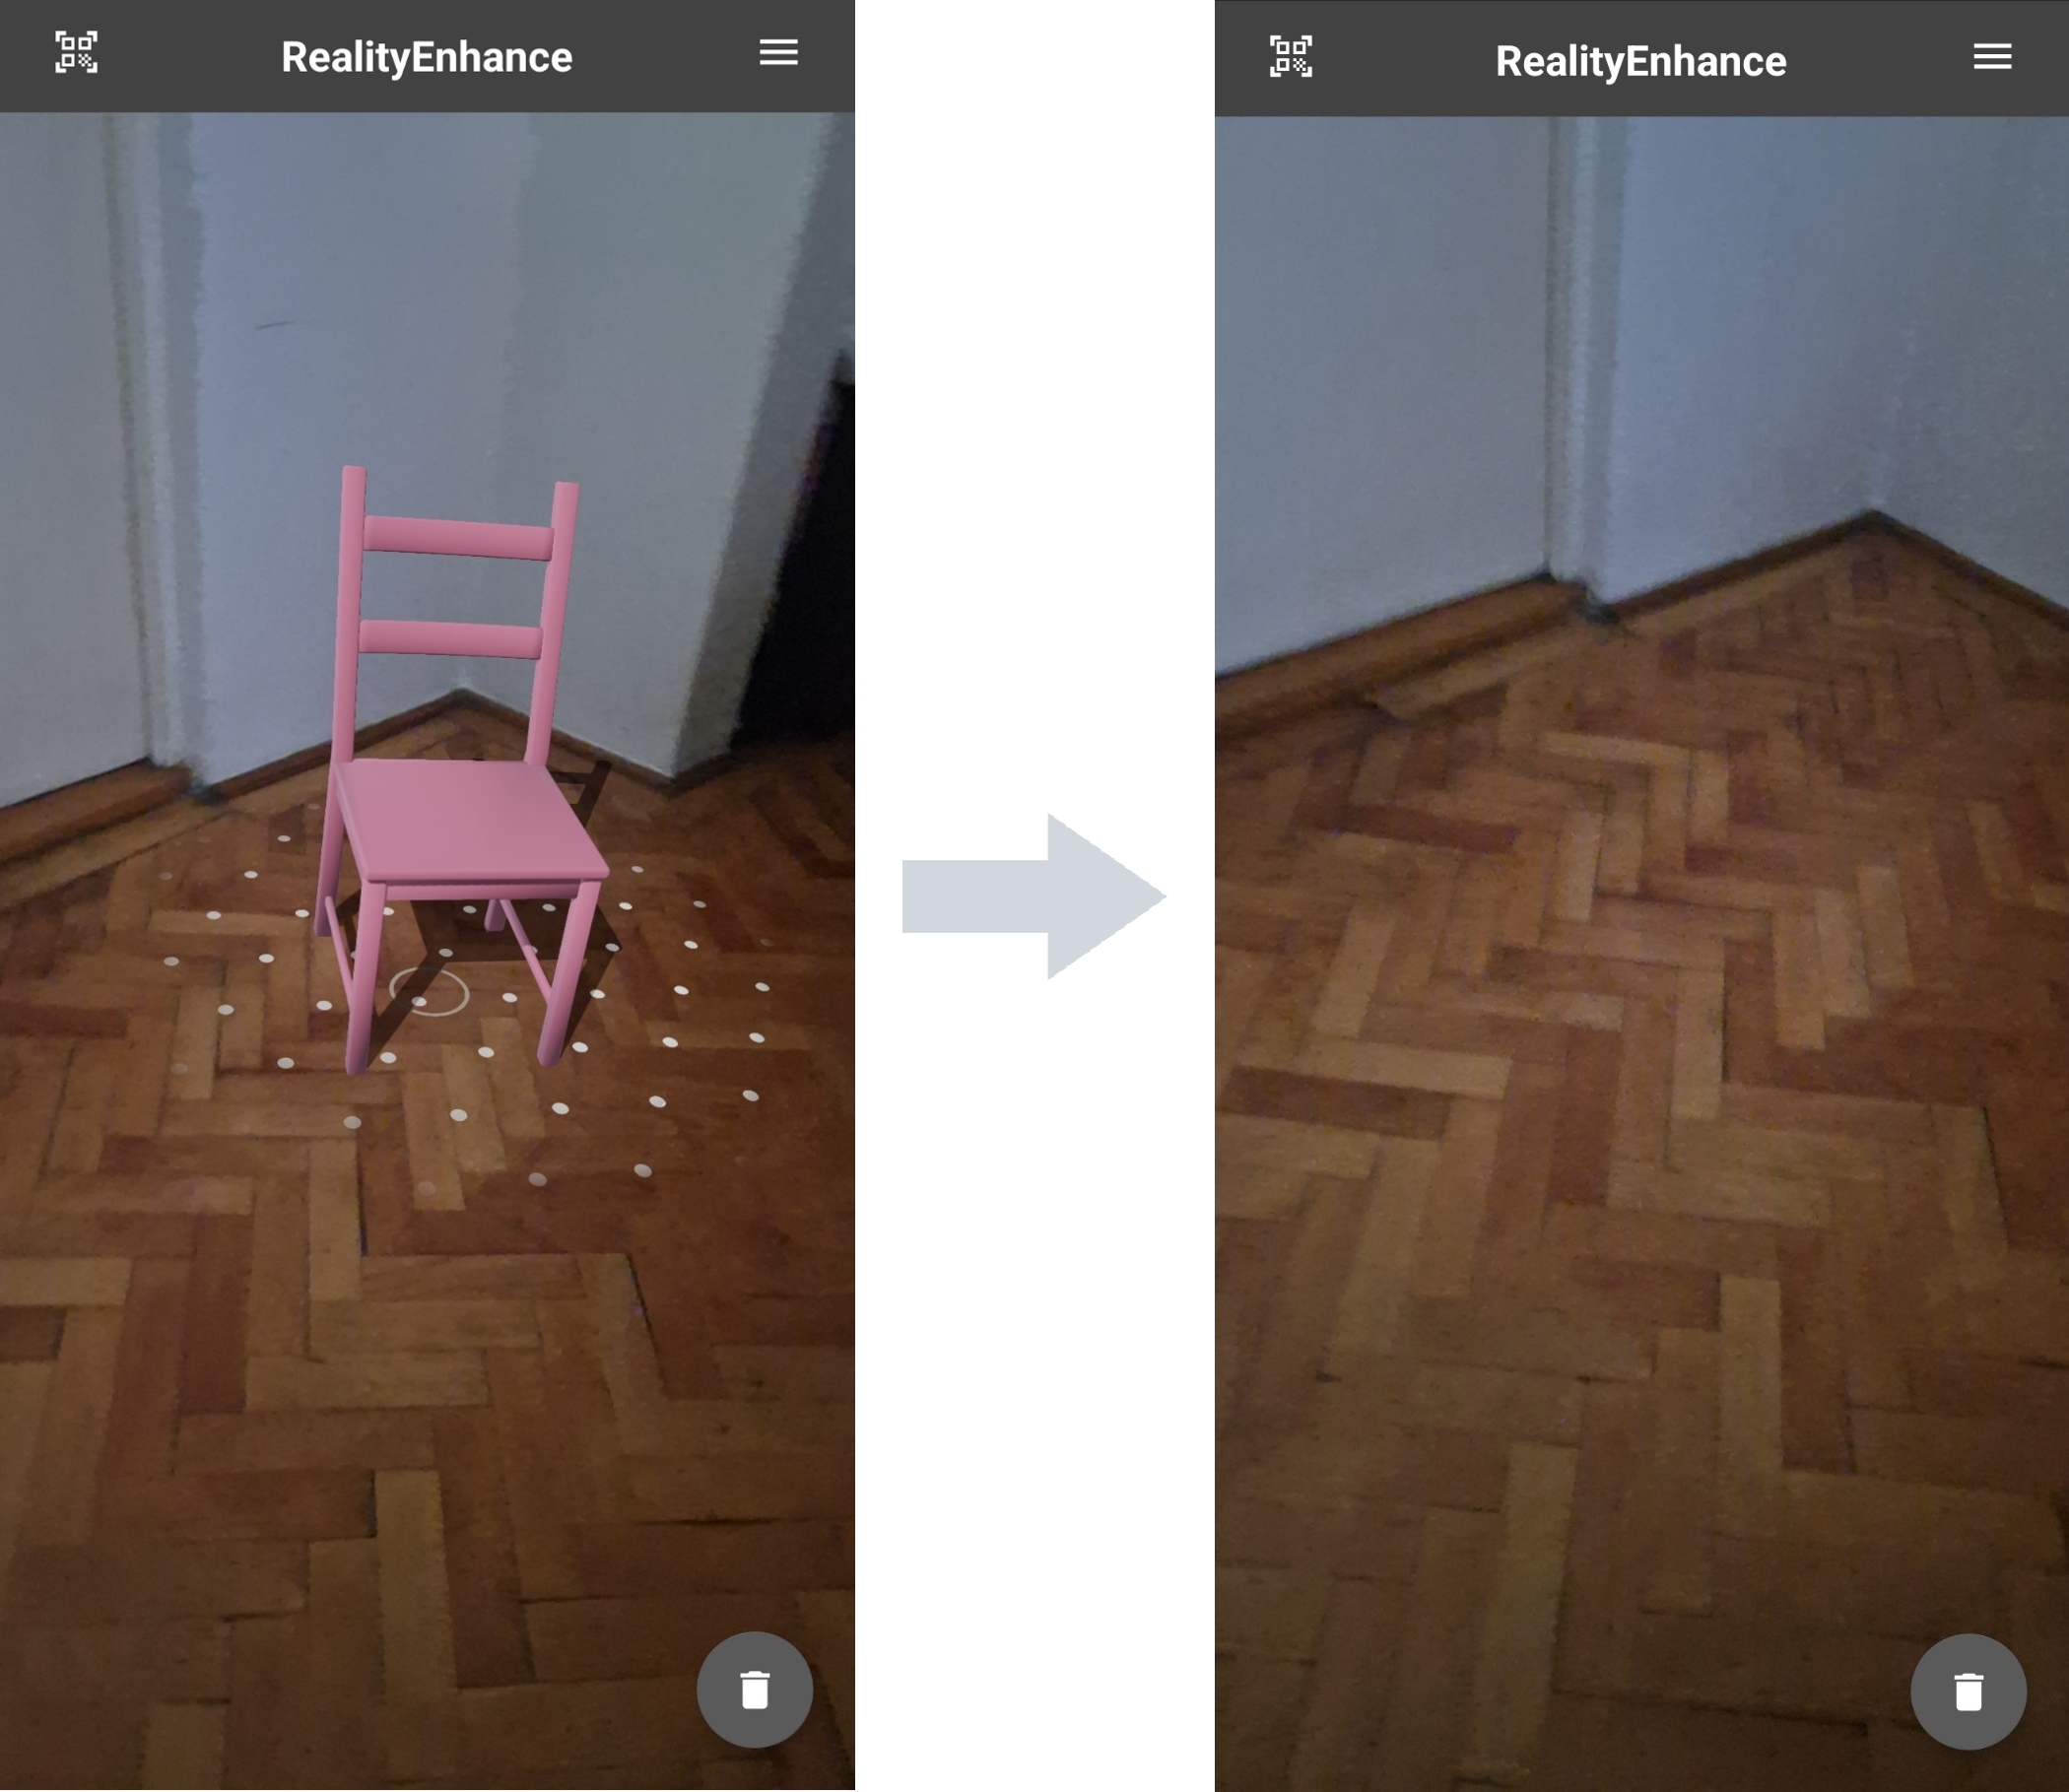
\includegraphics[width=1\textwidth]{img/App_screenshots/Model-removed.png}
        \caption{Removing a model}
        \label{fig:remove-a-model}
    \end{center}
\end{figure}

\pagebreak

\subsection{Resizing, moving and rotating a model}
The user is able to change the position of a \ac{3D} model by holding the model and dragging it across the screen; it is also possible to move the model by holding it and moving the smartphone.  The model can be resized by pinching the model with two fingers and it can be rotate the model with the same two fingers. It can be seen in Figure \ref{fig:Rezise and rotate a model} as an example of resizing and rotating a model. The gestures used to resize and rotate a model are the same gestures used to resize and rotate an image in the gallery application.

\begin{figure}[ht]
    \begin{center}
        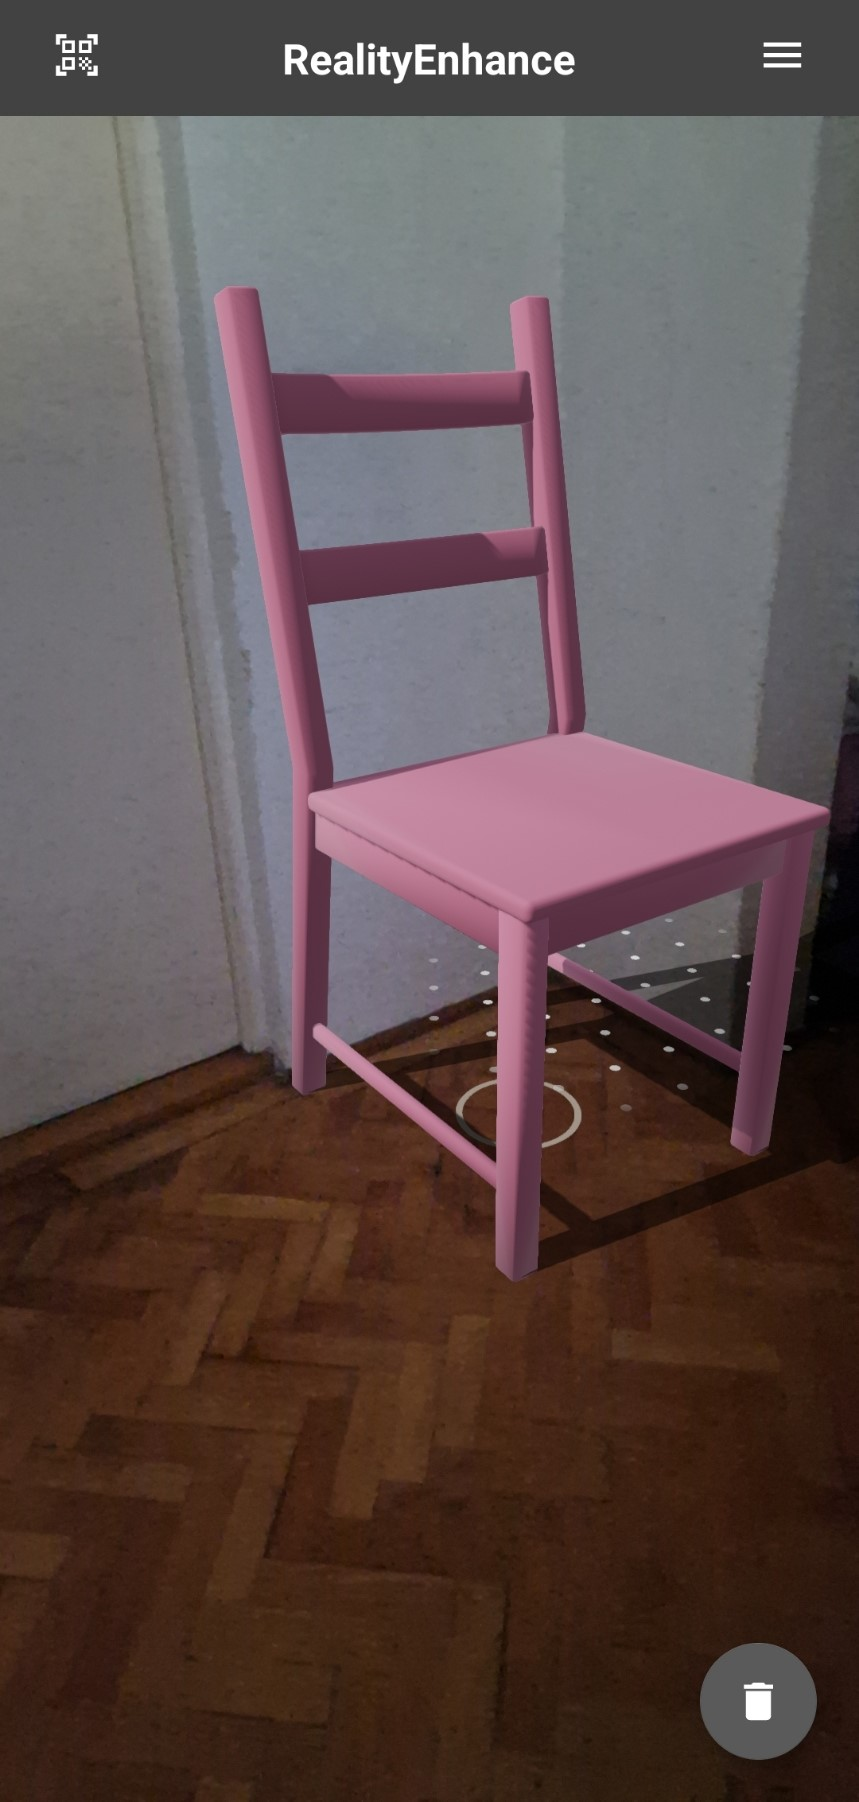
\includegraphics[width=0.4\textwidth]{img/App_screenshots/Size-rotation.jpg}
        \caption{Resized and rotated a model}
        \label{fig:Rezise and rotate a model}
    \end{center}
\end{figure}
\pagebreak

\subsection{Interacting with a model}
Some models will have a unique interaction with the user. Those models with access to the interactive feature are marked with a hat icon in the library, and when they are placed in the scene, the interaction button will appear at the bottom left of the screen.

As shown in Figure \ref{fig:Interactive model}, after the user clicks on the interaction button, the model of a geometrical cube changes from a whole cube to just the edges being visible. This interaction is just an example of what can be done with the interactive feature. Another example of an interactive model is a model of a LEGO man that will have a tutorial for assembling the LEGO figure as the interactive part.

\begin{figure}[ht]
    \begin{center}
        \subfigure{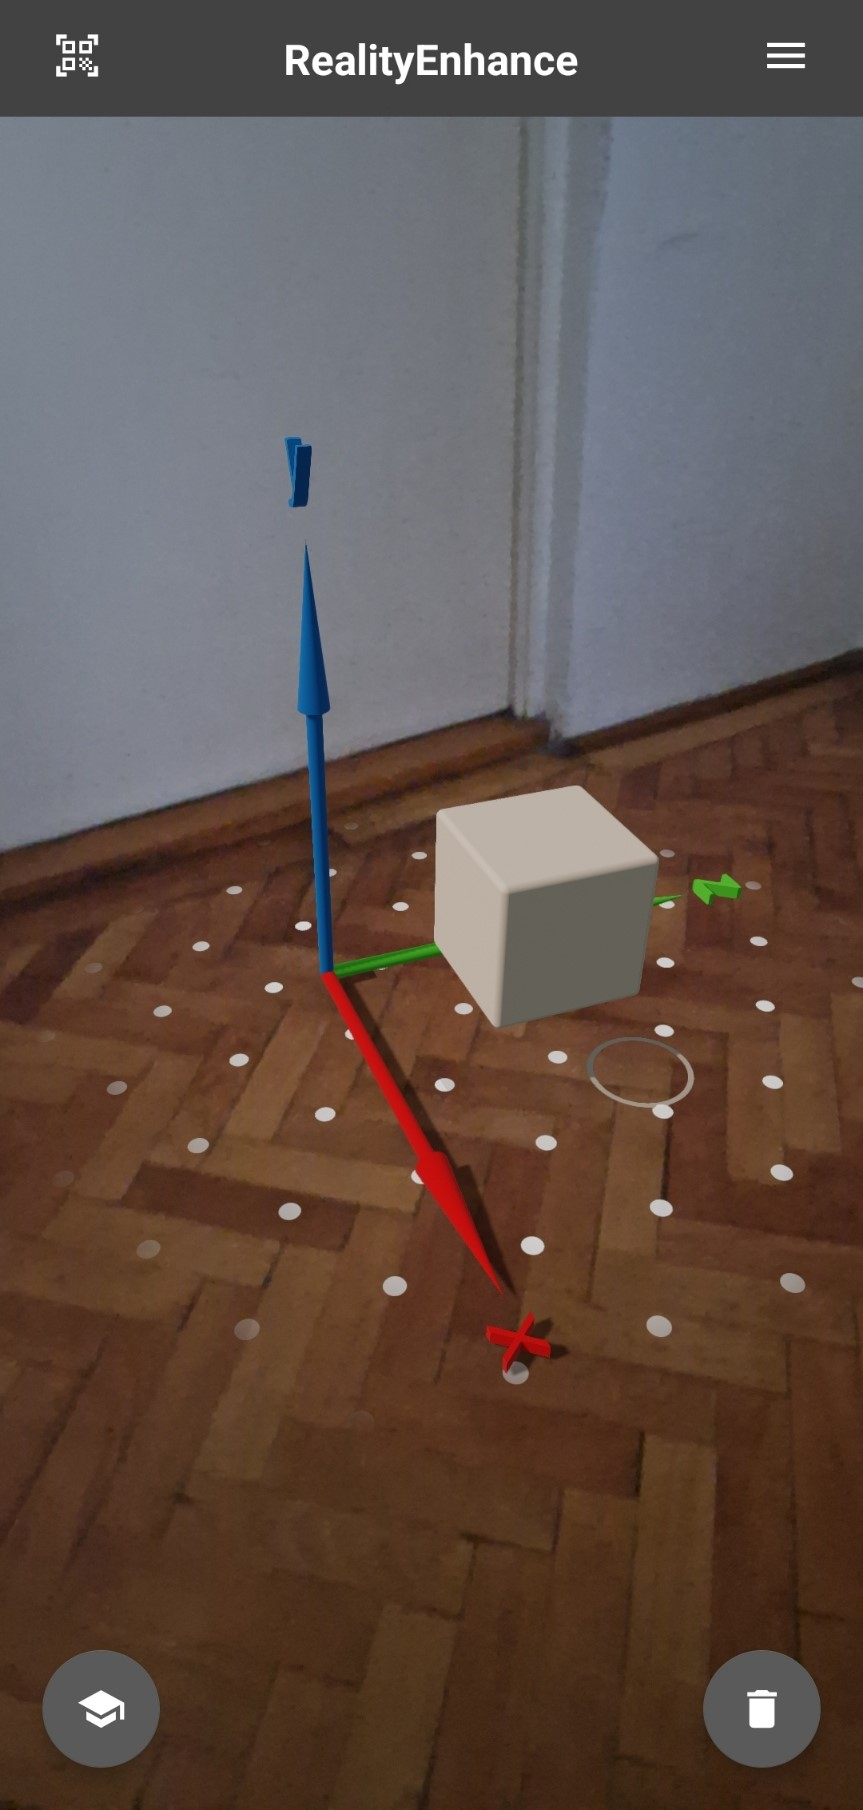
\includegraphics[width=0.4\textwidth]{img/App_screenshots/Interactive-model1.jpg}}
        \hspace{2cm} % Adjust the horizontal spacing between the images
        \subfigure{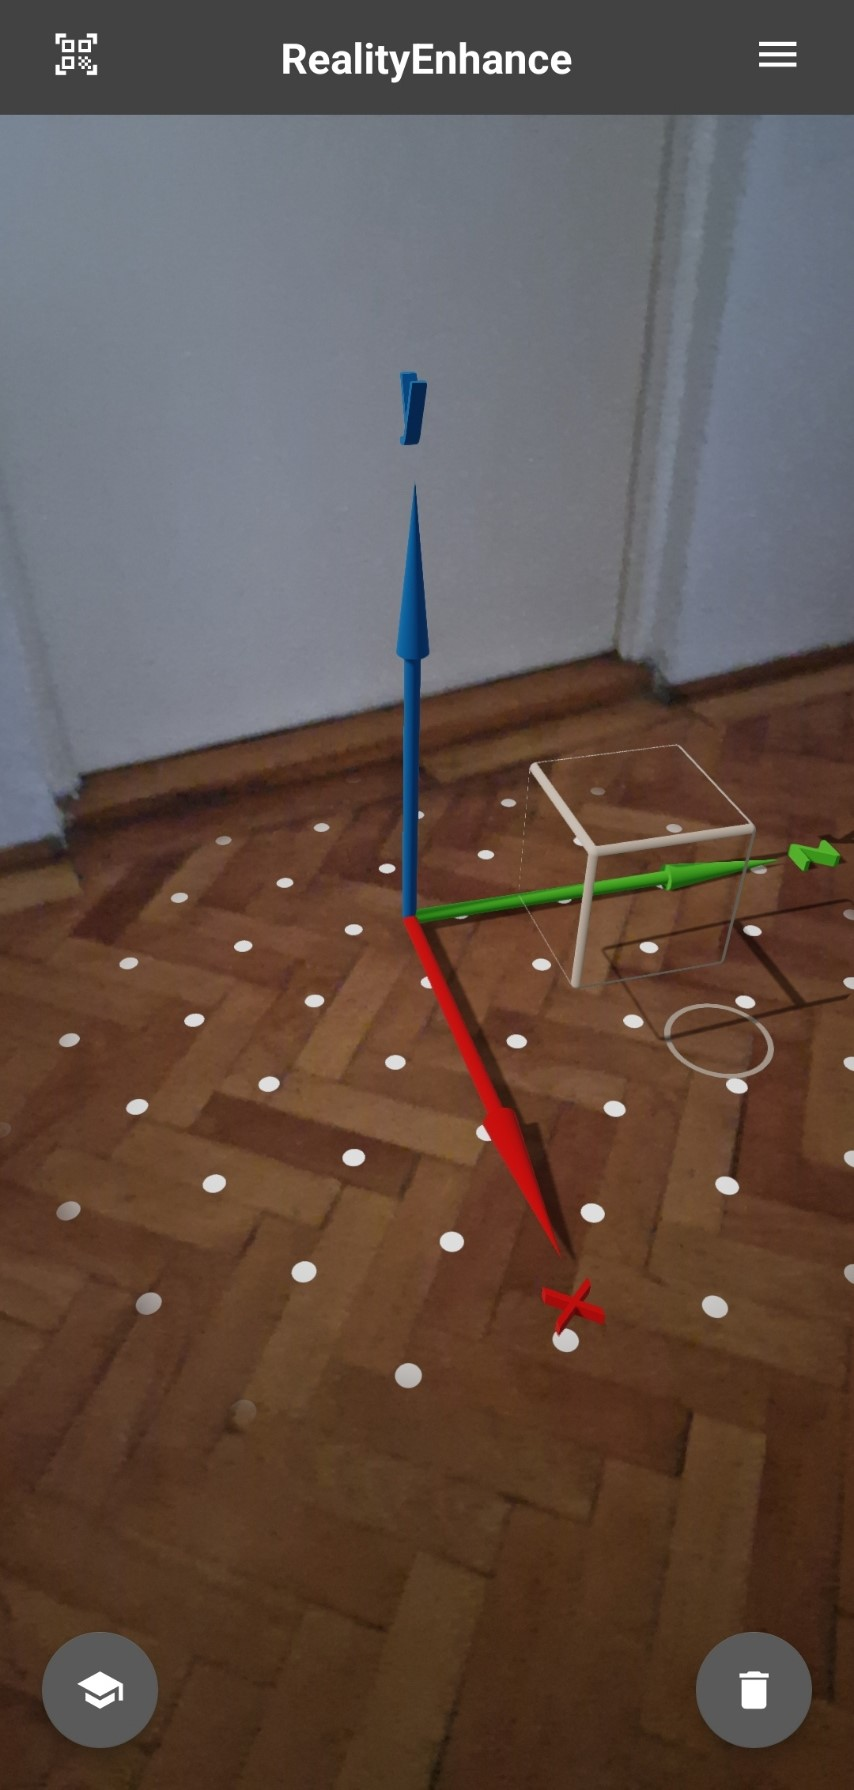
\includegraphics[width=0.4\textwidth]{img/App_screenshots/Interactive-model2.jpg}}
        \caption{Interactive model}
        \label{fig:Interactive model}
    \end{center}
\end{figure}
\pagebreak
